Para el desarrollo de cada Sprint, se utiliza una aplicación gratuita y Open Source llamada Taiga, la cual es una plataforma de gestión de proyectos para diseñadores ágiles.

Para comenzar a utilizar esta plataforma se deben registrar las historias de usuarios con su respectiva prioridad (etapa conocida como Product Backlog). Una vez realizado lo anterior, se proceden a crear los Sprint y por último se añaden las historias de usuarios a cada uno de estos tal como se muestra en la \textbf{Figura~\ref{fig: SprintBacklog}} y en caso de ser necesario, una historia del Prooduct Backlog puede ser subdividad para lograr un mejor enfoque y claridad en el desarrollo.

\begin{figure}[h!]
    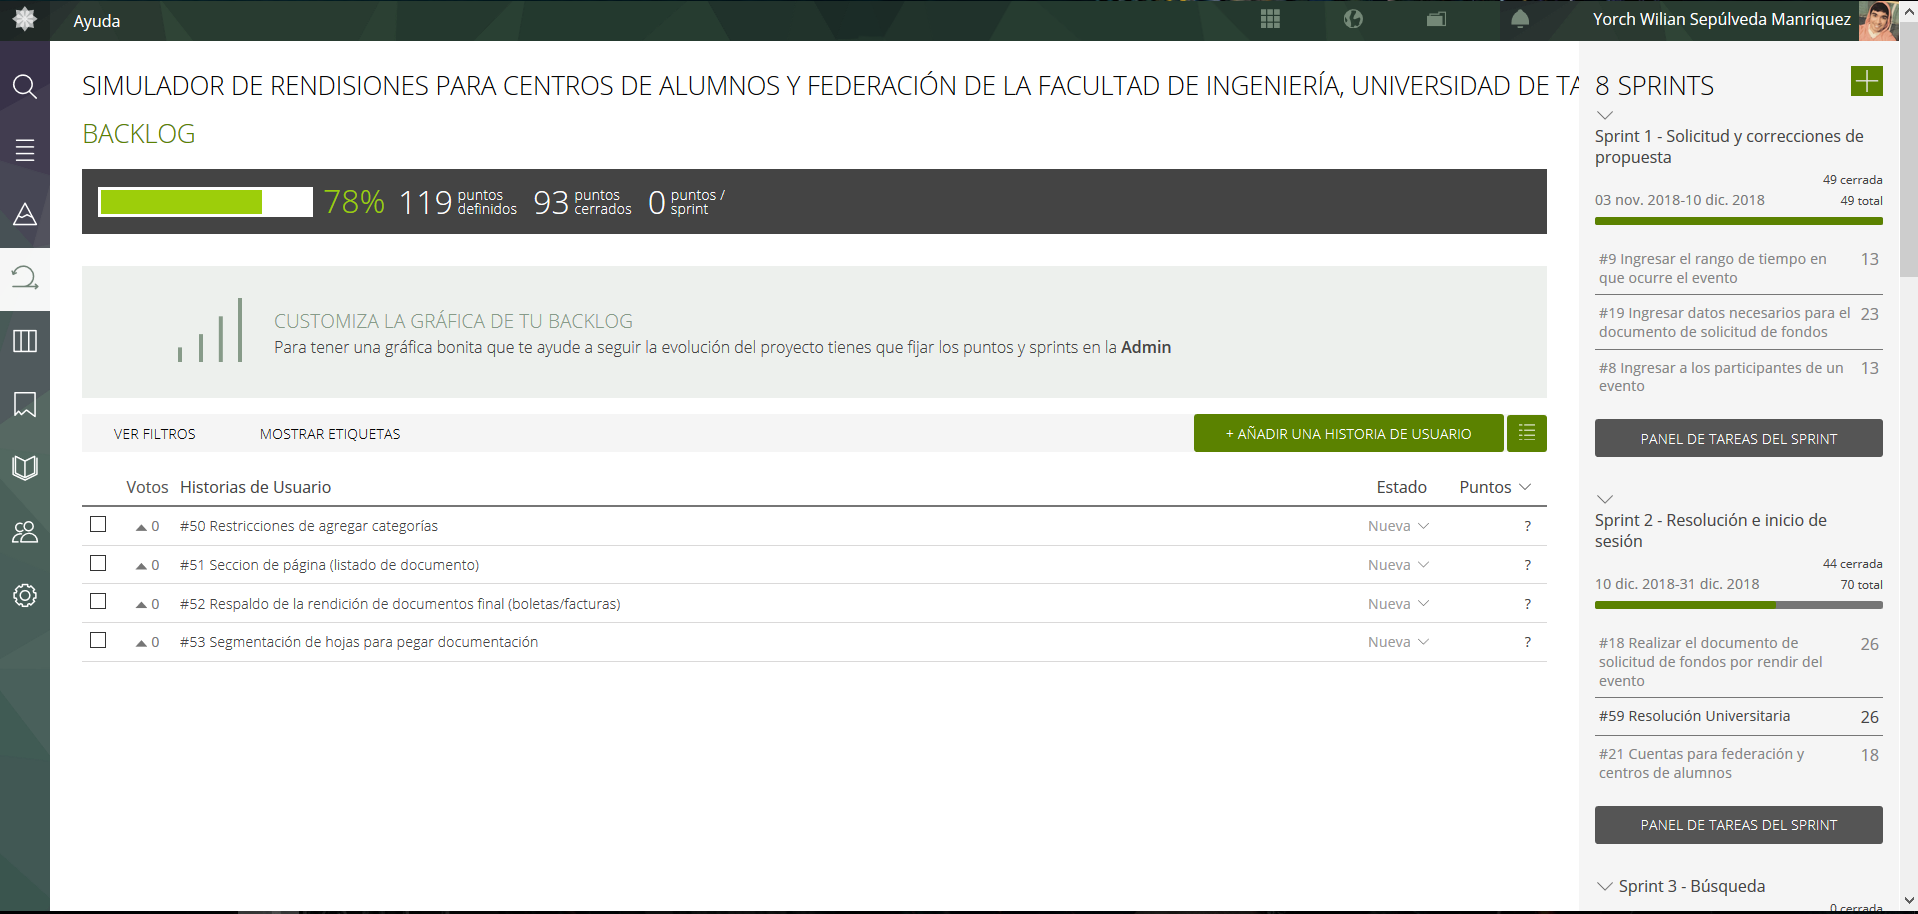
\includegraphics[width=\textwidth]{Imagenes/SprintBacklog.png}
    \caption{\label{fig: SprintBacklog} Sprint Backlog.}
\end{figure}

Dentro de cada Sprint hay un Kanban, el cual ayuda a organizar el desarrollo de cada historia de usuario realizada en el Sprint Backlog, en donde divide el trabajo en pequeñas tarjetas o tickets.

Dado lo anterior es que se divide el proceso de trabajo en cinco columnas como se muestra en la \textbf{Figura~\ref{fig: kanbanSprint}}, en donde se encuentra:

\begin{itemize}
    \item   \begin{description}
                \item[Nueva:] Se ingresan pequeñas tarjetas o ticket de trabajo que ayudan a realizar el cumplimiento de la historia de usuario 
            \end{description}

    \item   \begin{description}
                \item[En curso:] sección en donde se encuentran las tareas que se estan realizando
            \end{description}

    \item   \begin{description}
                \item[Lista para Testear:] columna en la que se encuentran las tareas terminadas y en proceso de aceptación
            \end{description}

    \item   \begin{description}
                \item[Cerrada:] área en donde se encuentran las tareas que han sido finalizada y aceptadas.
            \end{description}
    
    \item   \begin{description}
                \item[Necesita Información:] sección en donde se encuentran las tareas que no ha logrado culminarse debido a que falta información para su realización.
            \end{description}
\end{itemize}

\begin{figure}[h!]
    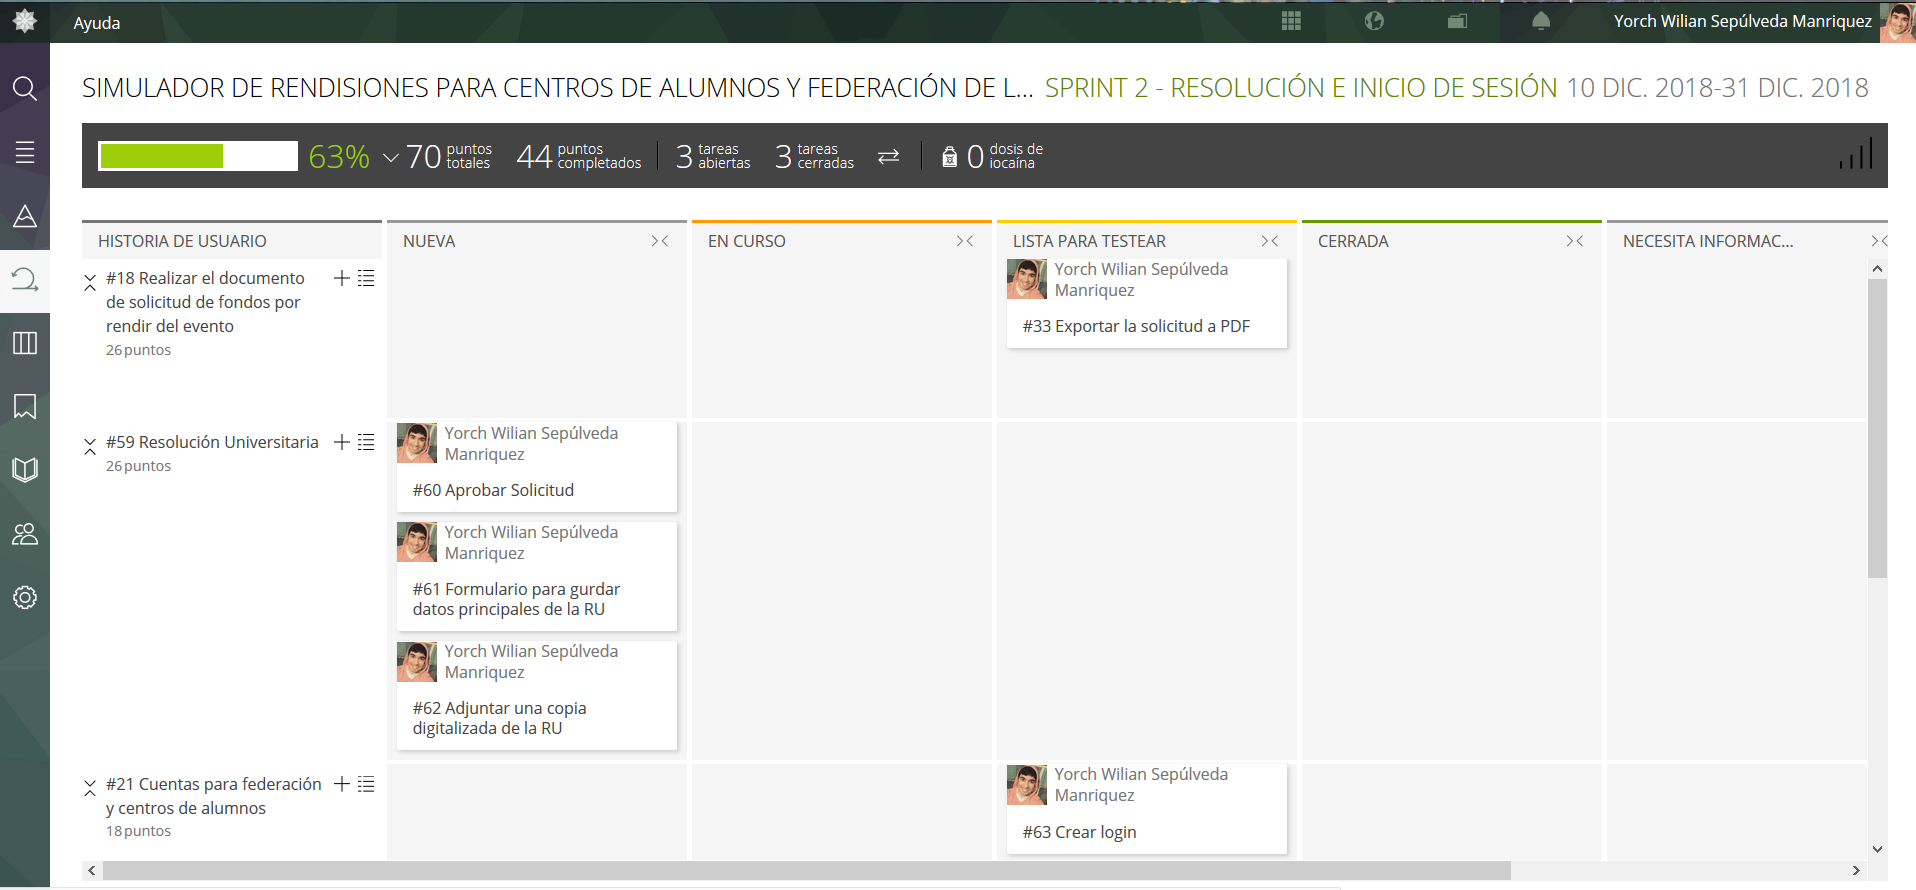
\includegraphics[width=\textwidth]{Imagenes/Kanban.png}
    \caption{\label{fig: kanbanSprint} Proceso de trabajo de un Sprint.}
\end{figure}

